\subsection{Long-slit spectroscopy mode}
\label{ssec:algo_lss_spectroscopy}

%-----------------------------------------------------------------------------------------
\subsubsection{Order background contamination removal}\label{ssec:orderbg}
Order background contamination may arise from internal straylight probably covering larger areas of the detector. Since it is expected to be low frequency only, its removal can be achieved by a low-order 2D polynomial fit 
\begin{equation}
    z = (a_0 + a_1x + a_2y + a_3x^2 + a_4x^2y + a_5x^2y^2 + a_6y^2 + a_7xy^2 + a_8xy ...)
\end{equation}
and a subsequent subtraction. The fitting points/regions must be chosen to be outside the \ac{LSS} order. Whereas these fitting points/regions can be chosen on fairly regular basis due to the straight order geometry in the \ac{LSS} mode, the degree of the polynomial depends on the actual straylight. This can be determined only during the testing phase when first real data are available.

%-----------------------------------------------------------------------------------------
\subsubsection{Order detection and rectification}\label{ssec:orderhandling}
The algorithms for order detection and rectification are adopted from \cite{pis02,pis21}.
In brief, the selection of pixels that may belong to spectral \ac{LSS} order is done by first smoothing each column and then selecting pixels above the median of the difference between the original
and the smoothed column, i.e. pixel $(x,y)$ is selected if
\begin{equation}
    I(x,y) > \bar{I}(x,y) + \mathrm{Median} ( I(x,y) - \bar{I}(x,y) ) .
\end{equation}
In the following a clustering analysis is performed, which associates connected groups of pixels. This is done scanning rows and columns and identifying neighbouring pixels selected in the previous step as belonging to the same cluster if $\delta x$ and $\delta y$ differ by at most 1. As spectral orders may be partitioned into different clusters because of e.g. detector defects, polynomial fits to the clusters are performed and the pairwise extensions of the fits to consecutive clusters are compared to identify which clusters are to be merged according to predefined criteria for the goodness of match. For each order, the detection algorithm yields a polynomial description of order location on the detector (the order center and its edges), an uncertainty estimate
for the fitted polynomial, and the first and last columns to be used during spectrum extraction. 
%The upper and lower edges of the orders are also traced and fitted by the order tracing algorithm using the pinhole frames with the flatfield lamp. 
Order rectification is achieved using the PyReduce algorithm described by \cite{pis21} that can account for both tilt and curvature of the slit image.   

%-----------------------------------------------------------------------------------------
\subsubsection{Spectroscopic flux calibration strategy}\label{ssec:fluxcal}
Flux calibration implies the conversion of ADUs to physical units. This is done by comparing the observed spectrum of a standard star with its reference spectrum as seen without atmospheric and instrument/telescope signatures, facilitating the response function to be determined. The response function describes the optical throughput of the optical system, i.e. the instrumental effect on the flux. In principle this is a standard procedure and in \ac{METIS} basically the same approach as described in the \ac{HDRL} will be closely followed.

\textcolor{red}{TBD: slit flux losses due to PSF (cf. MICADO)?????}


%-----------------------------------------------------------------------------------------
\subsubsection{Telluric absorption correction}\label{ssec:tellcorr}
Due to the dense molecular absorption arising from the Earth's atmosphere, nearly every \c{MIR} regime spectrum requires a correction for these telluric features. The required atmospheric transmission curve can be achieved either by specific observations of a telluric standard star (\ac{TSS}, the "classical" way) or by a modelling approach. \\
\paragraph{Classic \ac{TSS} approach:\newline}
A telluric standard star (\ac{TSS}) spectrum is taken ideally directly before/after the science observations near the science target position (or at least at the same airmass) to probe the same pathway through the Earth's atmosphere. This \ac{TSS}-spectrum is processed in the same way as the science spectrum (except the absolute flux calibration). To remove intrinsic stellar features this spectrum is corrected with a model spectrum of this \ac{TSS}. Finally its continuum is normalised to unity. The resulting normalised spectrum (ideally) only contains the fingerprint of the Earth's atmospheric absorptions and can be used for the telluric correction.\\
There are several sources for model spectra available:
\begin{itemize}
    \item Cohen set (\cite{coh99}): Set of 422 stellar model templates, mainly K and M giants. One of the standard sets in \ac{MIR}.
    \item The SPEX \ac{IRTF} Spectral library\footnote{\url{http://irtfweb.ifa.hawaii.edu/~spex/IRTF_Spectral_Library/}}: Set of observed stellar spectra (F to M-type, some carbon and S-type stars and L and T dwarfs) in the range $0.8...5.0\mu$m mostly at a resolving power of $R\equiv\lambda/\Delta\lambda\sim2,000$.
    \item Phoenix code\footnote{\url{https://phoenix.astro.physik.uni-goettingen.de/}}\cite{phoenix}:\\
\end{itemize}
Currently the \ac{METIS} team looks into that topic and maybe assembles a set of appropriate \ac{TSS} stars.

\paragraph{Modelling approach:\newline} In the last years the modelling method has evolved. It is based on radiative transfer modelling of the Earth's atmosphere (\cite{mf1, mf2, molecfit}\footnote{\url{https://www.eso.org/sci/software/pipelines/skytools/molecfit}}). A height model of the Earth's atmosphere containing information of pressure, temperature and the concentration of molecules in combination with a radiative transfer model and a molecular line list is used to determine the transmission of the Earth's atmosphere at the time of observations. The approach by fitting specific molecular absorption features in the science spectra. The best-fit transmission function is finally used for the telluric correction.\\

LSF identical + In case the model spectrum also contains absolute flux values, this star could also be appropriate for the absolute flux calibration.


models available: SPEX \\
Cohen \cite{coh99}\\
VISIR pipeline\footnote{\url{https://www.eso.org/sci/software/pipelines/}} \cite{visir_manual}


In the past years the approach of modelling transmission curves of Earth's atmosphere has made significant progress leading to versatile and mature software packages for the telluric correction. One of these packages is \texttt{molecfit}\footnote{\url{http://www.eso.org/sci/software/pipelines/skytools/molecfit}} (\cite{mf1, mf2}). This package is optimised for the ESO framework and ESO instruments and is also foreseen to be used for \ac{METIS}.\\
The outcome of the \ac{ELT} working group meeting of 2021-03-15 was that future instrument pipelines should include dedicated recipes based on the telluric correction \texttt{telluriccorr} library \cite{telluriccorr}. This package is based on \texttt{molecfit} and will be provided and maintained by \ac{ESO}. The telluric correction will be performed in three dedicated recipes as post-correction   and closely follow the approach as implemented in the \ac{KMOS} pipeline. The three steps comprise the fit of the telluirc features (e.g. \REC{metis_LM_lss_mf_model} for the LM range), the calculation of the transmission curve (e.g. \REC{metis_LM_lss_mf_calctrans}) and the application of the actual correction (e.g. \REC{metis_LM_lss_mf_correct}). For the determination of the \ac{LSF} we primarily rely on the possibilities as offered by the \texttt{telluricorr}/\texttt{molecfit} package, which is based on a fitting of the \ac{LSF} by a combination of a boxcar, Gaussian or Lorentzian. On basis of the commissioning data we will establish a parameter set providing a good starting point for the fits.\\
We also intend to enable the user to include a dedicated line kernel instead, in case a reliable kernel model can be determined with other (external) tools (e.g. a model-based convolution of an internal \ac{LSF}, the slit-widths and/or an \ac{AO} component). In addition, also external supplementary meteorological data (e.g. provided by an \ac{LHATPRO} radiometer) can be included if the \texttt{telluricorr}/\texttt{molecfit} package offers that possibility.

\begin{figure}[ht]
  \centering
  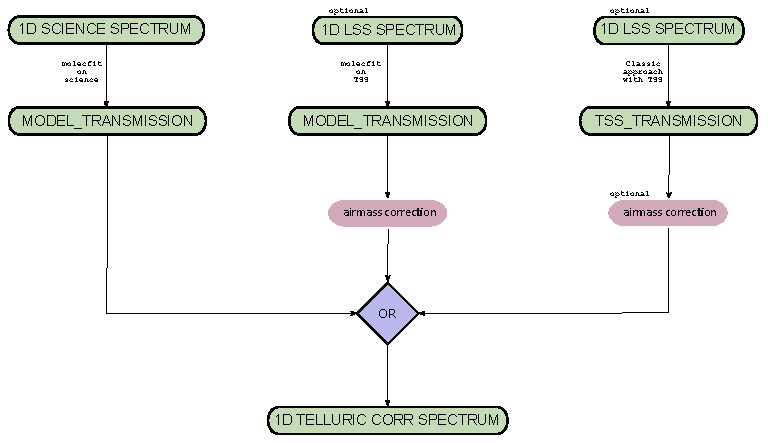
\includegraphics[width=0.9\textwidth]{figures/tell_corr_methods.pdf}
  \caption{Methods for the telluric correction to be included in the \ac{METIS} pipeline.}
  \label{Fig:tellcorrmethods}
\end{figure}

\textcolor{red}{TBD: Usage of TSS????}

%-----------------------------------------------------------------------------------------
\subsubsection{Object extraction and faint object spectroscopy}\label{sec:fospectro}
The object spectra will be extracted using the optimal extraction described by \cite{pis21} in order to maximized the \ac{SNR}. 
Faint objects will lead to additional requirements for the observation and the data reduction. For the target acquisition a blind offset from a reference source might become necessary in case the actual object cannot be detected directly. For the data reduction, manual interaction with the user is expected to be necessary to define the target position along the slit since automatic object detection algorithms (e.g. optimal extraction %\cite{hor86}) 
rely on a certain \ac{SNR}. This will be implemented as interactive actor in Reflex (or ESO-DPS).